\documentclass[]{book}

%\usepackage{url}
\usepackage{hyperref}
\usepackage[pdftex]{graphicx}
\usepackage[tikz]{bclogo}
\sloppy
\newenvironment{contentsmall}{\small}

\title{Csound System Documentation}
\author{Steven Yi}

\begin{document}
\maketitle

%===========================
\chapter{Introduction}

...

\section{Orientation}

\subsection{CMake Build System}

For Csound 6, we use the \href{http://www.cmake.org}{CMake} build
system. CMake is a meta-build system in that builds project files that
are then used with other build systems. This can produce files for
command-line build systems such as Make or
\href{http://martine.github.io/ninja/}{Ninja}, as well as build projects
for IDE's such as XCode, Eclipse, or KDevelop.

CMake organizes the build files into ones called CMakeLists.txt. Csound
has a top-level CMakeLists.txt that defines some useful functions, as
well as defines the build for libcsound. From there, other
CMakeLists.txt files are included into the top-level one that has build
information for other artifacts, such as command-line executables,
plugin libraries, and GUI applications.

\subsection{Dependencies}

\paragraph{Targets: libcsound, Executables, Plugin Libraries, and other
Libraries}

\subsection{Source Tree Walkthrough}

\begin{description}

\item[cs6] root of Csound 6

\item[cs6/include] public headers that will get distributed and used by host-applications
and plugin libraries

\item[cs6/H] private headers that are only used within libcsound itself

\item[cs6/Top] Contains source files for the parts that wrap the engine, including
argument parsing, module loading, CSD reading, CScore, and others

\item[cs6/Engine] Contains source files for the audio engine and compiler of Csound

\item[cs6/InOut] Contains source files for plugin libraries dealing with input and
output, particularly audio, midi, and graphs

\item[cs6/OOps] Contains source files for opcodes. Originally named for ``Original
Opcodes'', now contains mostly opcodes built-in to libcsound

\item[cs6/Opcodes] Contains source files for opcodes. Those that do not have external
library dependencies have been folded back into libcsound. Those with
external dependencies are built as separate opcode plugins.

\item[cs6/interfaces] Contains the source files for building the various interface wrapper
libraries (i.e.~Java, Python), as well as the C++ interface library.

\item[cs6/frontends] Contains the source files for building various frontends (i.e.~CsoundAC,
csoundapi\textasciitilde{}, beats).

\item[cs6/util] Contains the source files for the main csound-related utilities
(i.e.~pvanal, lpanal, dnoise, etc.). The files here are used to build
individual commandline programs, as well as altogether for the stdutil
plugin library.

\item[cs6/util1] Contains the source files for building various frontends (i.e.~CsoundAC,
csoundapi\textasciitilde{}, beats).

\item[cs6/installer] Contains the source code and build scripts for creating various
platform-specific installers.

\item[cs6/android] Contains example projects and build scripts for building Csound for
Android.

\item[cs6/iOS] Contains example projects and build scripts for building Csound for iOS.

\end{description}


%===========================
\chapter{High-Level Architecture}

\begin{figure}[htbp]
\centerline{\framebox{
        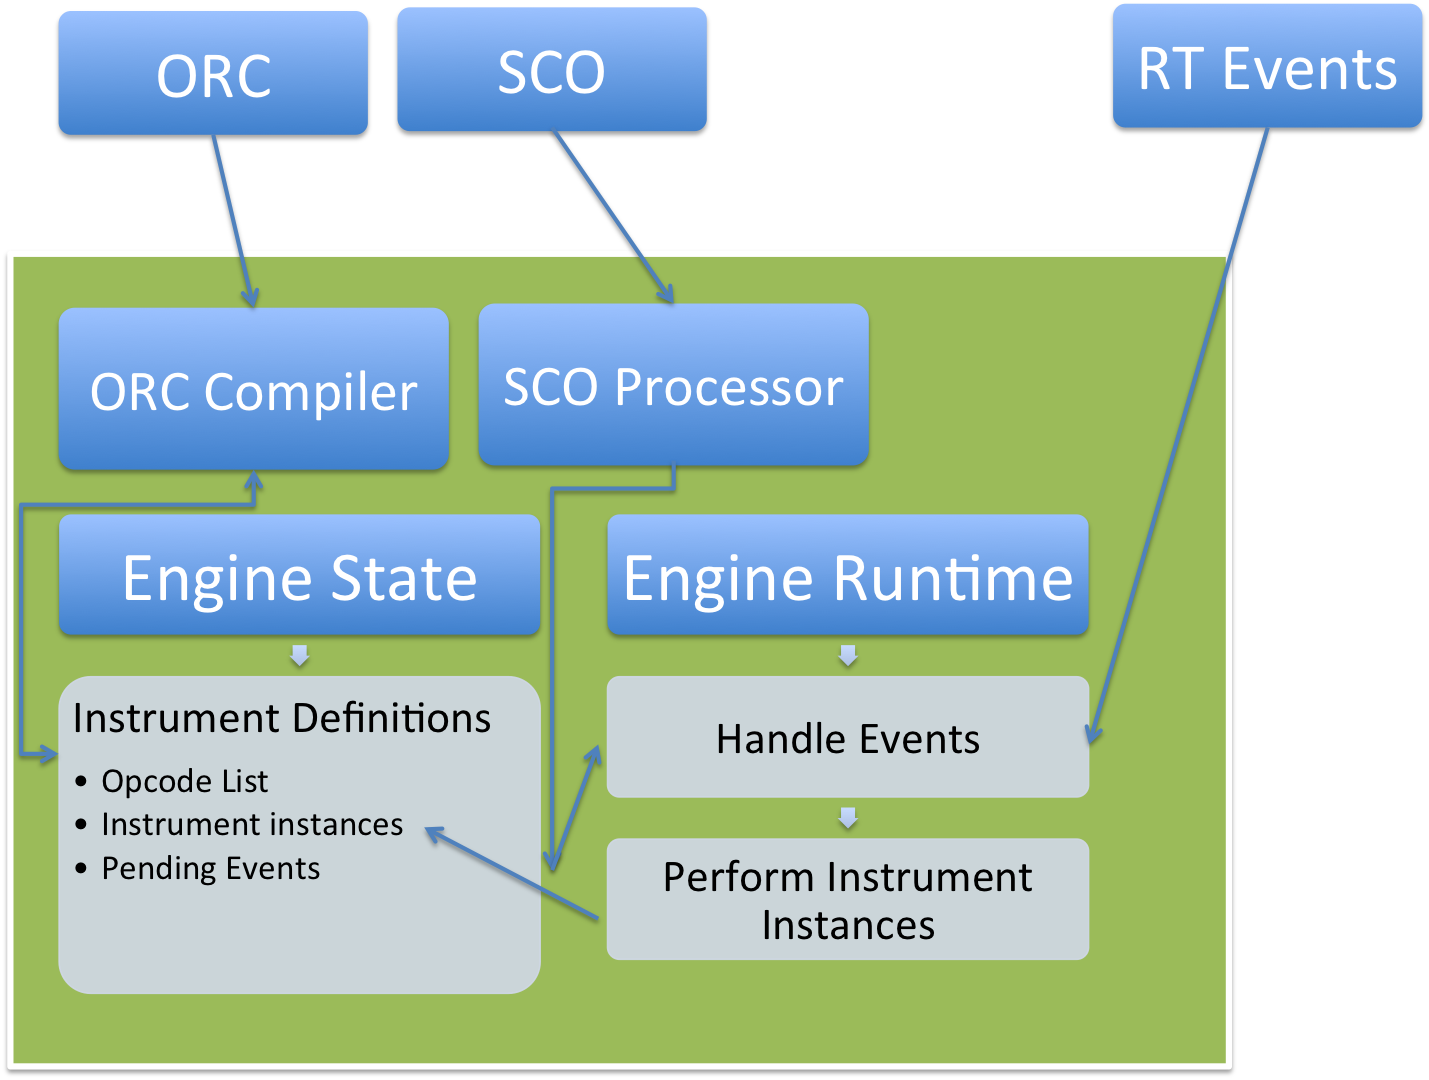
\includegraphics[width=0.8\textwidth]{images/overview.png}}}
\caption{Csound System Architecture Overview}
\label{overview}
\end{figure}

The architecture of Csound follows in the tradition of Music-N. In general, Csound ORC code is used to define \emph{Instruments}, which are then instantiated at run-time by Csound SCO events, MIDI events, Remote events, or API calls. Instruments in turn are made up of a series of \emph{Opcodes}, which are the Unit-Generators of Music-N heritage.

In further detail, Csound Orchestra code is used to define instrument templates.  The ORC code, as text, goes through the Csound Orchestra Compiler, and at the end is compiled into INSTRTXT instances that are held in a linked-list.  The information held in INSTRTXT instances include information relevant for runtime instantiation, initiation, and performance of an instrument.  This information includes what opcodes are used and in what order for both initialization and performance time, what variables are required (including the names of the variables as well as their types), as well as how the memory for variables and opcodes are all hooked up to teach other.  

For traditional Music-N systems that were not capable of accepting realtime events, a score was used as the single source of events that would trigger changes to the state of the system, such as initializing new instances of instruments or creating new function tables. In Csound, this system is still in place with the processing of SCO code at compile-time, but it also augmented with the processing of events at runtime. Before run-time, if a Csound SCO block is passed to the Score compiler, it will be processed, sorted, time-warped, and re-written as a well-formatted string.  This well-formatted string, read in using the CORFILE mechanism, represented the notes of a note-list composition.  

In addition to the well-formatted SCO, realtime events can also affect the state of the system.  In general, the main performance function, kperf(), is used to process pending events (sensevents()), expire current instances (timeexpire(), beatexpire()), as well as run active instances.  In sensevents(), events that a processed are new SCO events that have arrived via STDIN pipe, SCO events from the API (csoundReadScore()), MIDI events, as well as Remote events.

At runtime, kperf() is called once per-audio buffer.  The buffer is of ksmps size.  Within that kperf() call, sensevents() is called to update the state of Csound and active instruments are performed.  In general, an application such as the csound command-line executable or an API host application will repeatedly call kperf().  Csound will continue to run until an end condition is met: end of Score, end of MIDI file (if MIDI file was supplied at commandline), encounter of the 'e' event, or an API application stops Csound.  

%===========================
\chapter{Prelude to Processing}

\section{Csound Configuration (Commandline Args/Options)}

\section{ORC/SCO/CSD Input}

Text is read through one of two primary paths:

\begin{itemize}
\itemsep1pt\parskip0pt\parsep0pt
\item
  from files
\item
  from memory
\end{itemize}

Both of the paths actually filter through the CORFILE system\ldots{}

%===========================
\chapter{Orchestra Compiler}

\section{Introduction}

\section{Compiler Phases}

\begin{figure}[htbp]
\centerline{\framebox{
        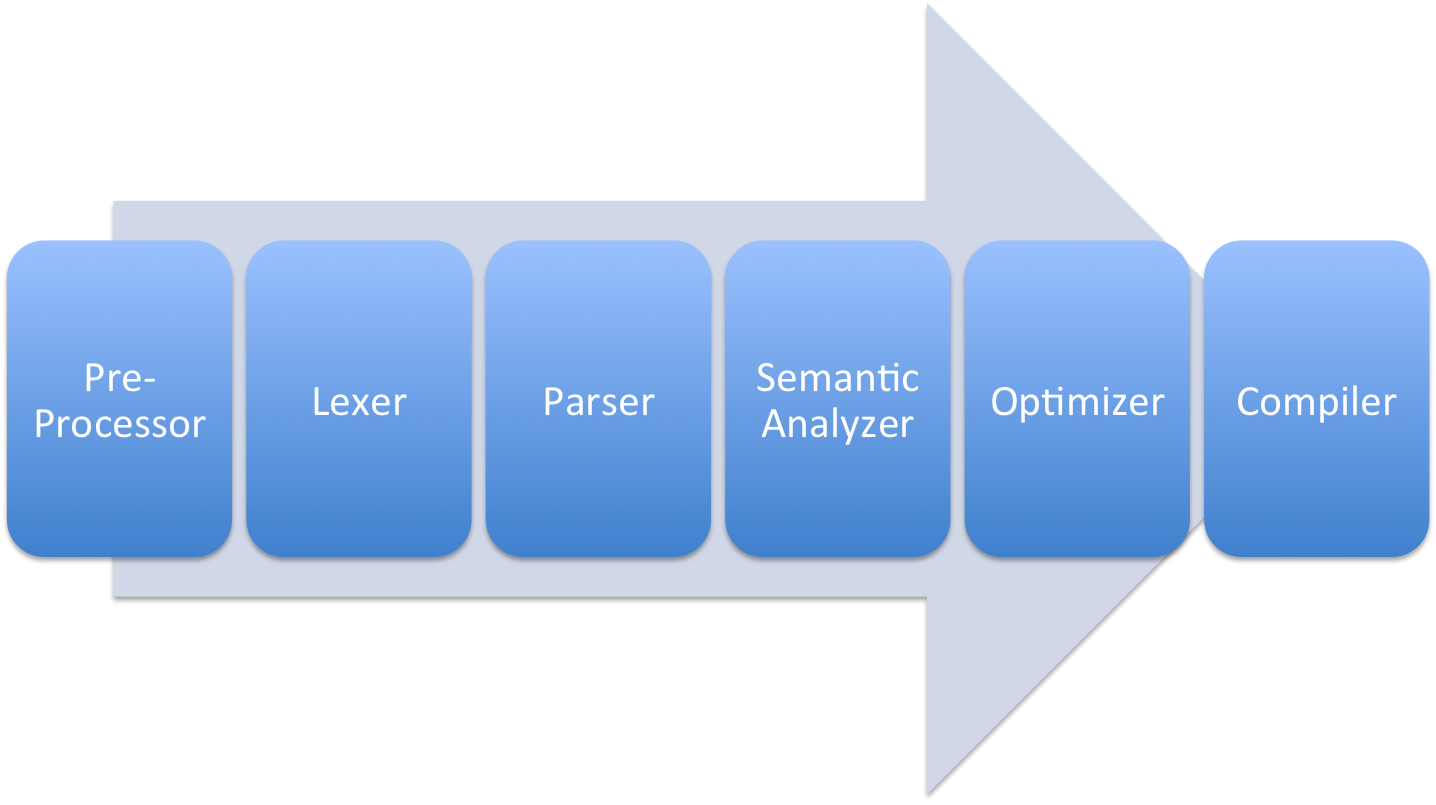
\includegraphics[width=0.8\textwidth]{images/compiler.png}}}
\caption{Csound Compiler Phases}
\label{overview}
\end{figure}

Csound compiler is separated into a number of distinct phases, as illustrated by the figure above. The following subsections will discuss each phase of the compiler.  It will include relevant data structures, functions, and files to consult.  

\subsection{CORFIL}

The CORFIL mechanism is an implementation of an in-memory file system. ...

\subsection{Pre-Processing}

% using bclogo, but would be happy to switch to something else too
\begin{bclogo}[couleur=blue!30,arrondi=0.1,ombre=true,logo=\bcetoile]
{Important Files}
Engine/csound\_pre.l (Flex file)
\end{bclogo}

The Orchestra Pre-Processor is responsible for processing the following things:

\begin{itemize}
  \item \#include - processing to include text from an external file
  \item \#define - reading in Orchestra Macro definitions
  \item \#undef - un-define a macro
  \item \$MACRO - processing Orchestra Macro usages
  \item \#ifdef, \#ifndef, \#else, \#end - conditionally include text
\end{itemize}

The pre-processor is generated using \href{http://flex.sourceforge.net/}{Flex}. It is given text and the expanded processed text is returned (this is done with the text wrapped in a CORFIL). The call to csound\_prelex() is done within new\_orc\_parser.c::csoundParseOrc(), with most of the implementation of the pre-processor utility functions done within csound\_pre.l.

\subsection{Lexer}

\begin{bclogo}[couleur=blue!30,arrondi=0.1,ombre=true,logo=\bcetoile]
{Important Files}
Engine/csound\_orc.l (Flex file)
\end{bclogo}

The lexing phase reads in a stream of characters and breaks them up into
tokens. (Lexers are also known as\emph{scanners} or \emph{tokenizers}.)
Csound uses the \href{http://flex.sourceforge.net/}{Flex} tool to
generate its lexing code. The source for this is found in
Engine/csound\_orc.l.


\subsection{Parser}

\begin{bclogo}[couleur=blue!30,arrondi=0.1,ombre=true,logo=\bcetoile]
{Important Files}
Engine/csound\_orc.y (Bison file)
\end{bclogo}

The parsing phase uses the tokens generated from the lexing phase and
uses rules defined in a \emph{grammar} to structure the tokens into a
TREE. The parsing code was originally done with hand-written code, but
is now generated using the
\href{http://www.gnu.org/software/bison/}{Bison} parser-generator tool.
The source for this is found in Engine/csound\_orc.y.


\subsection{Semantic Analysis}

\begin{bclogo}[couleur=blue!30,arrondi=0.1,ombre=true,logo=\bcetoile]
{Important Files}
Engine/csound\_orc\_semantics.c 
Engine/csound\_type\_system.c 
Engine/csound\_standard\_types.c 
\end{bclogo}

\subsubsection{Type System}

\subsubsection{Lookup}

\subsubsection{Expressions}

\subsubsection{Blocks}

\subsubsection{Compiler}

\section{Runtime Data Structures}

Instruments, Opcodes, Instrument Instances, Opcode Instances

\subsection{Labels, Block Expressions}

\subsection{Expression Expansion}

\subsection{Transactional Compilation}


%===========================
\chapter{Score Compiler}

\subsection{Event Parsing}

\subsection{Score Sorting}

\begin{center}\rule{3in}{0.4pt}\end{center}


%===========================
\chapter{Runtime}

\section{Introduction}

\section{Instrument Instance Lifecycle}

\section{Performance}

\section{Scheduler and senseEvents}

\subsection{Realtime Events}

\section{SCO}

\section{MIDI}

\section{Channels}


%===========================
\chapter{Other Features}

\section{Subinstruments and User-Defined Opcodes}

Subinstruments is a feature that allows one instrument to instantiate, run, and transfer values to/from another instrument instance. This feature was later modified as the User-Defined Opcode system, which allows users to create new opcodes using Csound ORC code. Internally, UDO's are stored as instrument definitions. They are performed in the same manner as an instrument in regards to there being a linked list of opcodes that are called at init- and performance-time.  

In general, Subinstruments differ from UDO's in that they do not add OENTRY's to the opcode table.  Instead, the subinstr and subinstrinit opcodes are used.  These opcodes will search the list of instrument definitions directly using the instrum or "instrname" argument given to the opcode. Once found, the instantiation is done using the instrument definition.  On the other hand, UDO's do add OENTRY's to the opcode table. This allows the name of the UDO to be used within orchestra code directly as an opcode name, rather than using subinstr and subinstrinit for all calls to the code.

The UDO system is described below. The primary code for UDO's and Subinstrument calls are contained within Engine/insert.c.

\subsection{Parsing of UDO's}

\subsection{Instantiation of UDO's}

\subsubsection{Interaction of internal state and arguments}

\subsection{Performance of UDO's}

\subsection{Other Notes}

\subsubsection{Opcode Overloading}


%===========================
\chapter{API and Wrappers}



%===========================
\chapter{Developer Information}

\section{Csound Testing}

The csound6/tests folder contains various forms of tests for Csound. The
tests are generally written to aid development, testing that new code
functions as expected and that they handle errors correctly. The
following describes the various forms of tests.

\subsection{tests/commandline}

This folder contains CSD's that get run by a python test
runner(test.py). These are generally used for testing the compiler and
can be considered integration tests. These can be run from the CMake
generated build file, i.e. ``make csdtests''.

Note: Some tests in the tests/commandline folder are not added to the
test suite. These are generally ones that people have contributed to
illustrate a bug, and were used during debugging. It is useful to have
these around and ideally we will extend the test suite to do runtime
testing as well as compiler testing.

\subsection{tests/c}

This folder contains unit tests written in C, using the CUnit library.
Currently there are tests for various parts of the compiler and some API
methods. These tests serve to help ensure we didn't break something
moving forward, and also act as a documentation on how functions are
used. These can be run from the CMake generated tests using ``make
test'' or calling ``ctest''.

\subsection{tests/python}

This folder is intended for tests of the Csound API using Python. The
idea is that it would be useful to test from a host language to make
sure our assumptions about the C API still work from a host language.

\end{document}
